\documentclass[11pt,oneside]{amsart}
\usepackage[margin=1in]{geometry}
\usepackage{amssymb,parskip,mathtools,microtype}
\usepackage[shortlabels]{enumitem}

\theoremstyle{definition}
\newtheorem{problem}{Problem}

\newcommand{\bC}{\mathbb{C}}
\newcommand{\bF}{\mathbb{F}}
\newcommand{\bQ}{\mathbb{Q}}
\newcommand{\bR}{\mathbb{R}}
\newcommand{\bZ}{\mathbb{Z}}
\newcommand{\bE}{\mathbb{E}}
\newcommand{\eps}{\varepsilon}

\DeclareMathOperator{\Var}{Var}
\let\Re\relax
\DeclareMathOperator{\Re}{Re}
\let\Im\relax
\DeclareMathOperator{\Im}{Im}
\DeclareMathOperator{\Arg}{Arg}
\DeclareMathOperator{\ord}{ord}
\DeclareMathOperator{\Res}{Res}

\title{MATH4460 Spring 2023\\
Final Exam}
\author{Thursday, May 11, 2023}

\begin{document}
\maketitle

Name: \underline{\hspace{6cm}}

This exam is open notes, but calculators are not allowed. There are 100 points total in this exam. If you do not manage to solve a problem, show a strategy you tried and a reflection on why it did not work, for partial credit.

\begin{problem}
\leavevmode\begin{enumerate}[(a)]
  \item (5 points) Decompose $\dfrac{3z^2}{z^3+1}$ into partial fractions.
        \vfill
  \item (5 points) Let $f(z)=z^2+i$. Let $a_0=0$ and $a_n=f(a_{n-1})$ for $n\geq 1$. Prove that the sequence $(a_n)_{n\geq 0}$ is bounded.
        \vfill
        \textbf{Bonus} (1 point). What does part (b) say about the Mandelbrot set?
        \raisebox{-0.45\height}{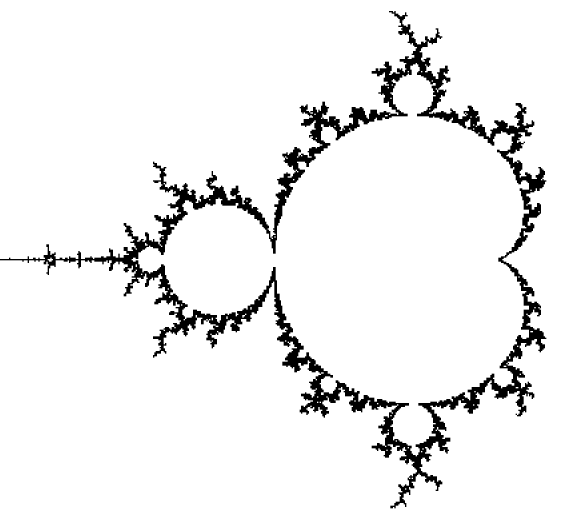
\includegraphics[width=3cm]{mandelbrot.png}}
        \vspace{2cm}
\end{enumerate}
\end{problem}

\newpage

\begin{problem}
  \leavevmode\begin{enumerate}[(a)]
    \item (5 points) Prove or give a counterexample: If $f(z)$ and $g(z)$ have a pole of order 2 at $z=a$, then $f(z)+g(z)$ also has a pole of order 2 at $z=a$.
    \vfill
    \item (5 points) Prove or disprove: There exists a sequence $(z_n)_{n\geq 0}$ of complex numbers such that both of the following hold:
    \begin{itemize}
      \item $e^{1/z_n}=-2023$ for all $n$.
      \item $\lim_{n\to\infty}z_n=0$.
    \end{itemize}
    \vfill
  \end{enumerate}
\end{problem}

\newpage

\begin{problem}
  Let $\gamma$ be the square with corners $\pm 2023\pm 2023i$, oriented counterclockwise.
  \begin{enumerate}[(a)]
    \item (3 points) Find
    \[\int_\gamma \frac 1{z^2+2024^2}\,dz.\]
    \vfill
    \item (3 points) Find
    \[\int_\gamma\frac 1{(z^2+2024^2)(z-2022)^2}\,dz.\]
    \vfill
    \item (4 points) Find
    \[\int_\gamma \frac {e^z}{e^z-2}\,dz.\]
    You may use the fact that $\frac{2023}{2\pi}\approx 321.97$.
    \vfill
  \end{enumerate}
\end{problem}

\newpage

\begin{problem}
\leavevmode\begin{enumerate}[(a)]
  \item (5 points) Sketch, in the complex plane, the set $\{e^z:z\in\bC\text{ and }\Re z=2\}$.
        \vfill
  \item (5 points) Let
  \[f(z)=\frac{e^{\frac 1{z+8}}}{(z-1)(z^2-1)(z^3-1)(z^4-1)}.\]
  Classify the singularities of $f$ in the extended complex plane $\widetilde\bC$, and give the order of each non-essential singularity.
        \vfill
\end{enumerate}
\end{problem}

\newpage

\begin{problem}
\leavevmode\begin{enumerate}[(a)]
  \item (4 points) Solve the equation $z^4+z^2+1=0$. Express the solutions as powers of $\omega\coloneqq e^{\pi i/3}$.
        \vfill
  \item (6 points)
        Calculate
        \[\int_{-\infty}^\infty \frac 1{x^4+x^2+1}\,dx.\]
        \vfill
        \vfill
\end{enumerate}
\end{problem}

\newpage

\begin{problem}
  \leavevmode\begin{enumerate}[(a)]
    \item (4 points) What is the Laurent series of $e^z/(z-2)^4$ around $z=2$?
    
    \emph{Hint}: $e^z=e^2\cdot e^{z-2}$.
    \vfill
    \vfill
    \item (1 point) Based on part (a), what is the residue of $e^z/(z-2)^4$ at $z=2$?
    \vfill
    \item (5 points) What is the disk of convergence of the power series of $f(z)=1/(z^4+16)$ around $z=-1$?
    
    \emph{Protip}: Don't compute the series. The first few terms are $\frac 1{17}+\frac 4{289}(z+1)-\frac{86}{4913}(z+1)^2+\cdots$ but this will not help.
    \vfill
    \vfill
  \end{enumerate}
\end{problem}

\newpage

\begin{problem}[10 points]
Liouville's theorem states that a bounded entire function is constant. Prove the stronger statement that a bounded holomorphic function on $\bC-\{a_1,a_2,\dots,a_n\}$, where $\{a_1,a_2,\dots,a_n\}$ is a finite set of complex numbers, must be constant.
\end{problem}

\newpage

\begin{problem}[10 points]
  Let $\gamma$ be the curve
  \[z(t)=e^{10(\cos t+i\sin t)}, 0\leq t\leq 2\pi.\]
  Prove, non-graphically, that the winding number of $\gamma$ around the origin is 0.
\end{problem}

\newpage

\begin{problem}
  \leavevmode\begin{enumerate}[(a)]
    \item (5 points) Prove that for $\Re s>1$,
    \[\sum_{n=1}^\infty\frac{(-1)^{n+1}}{n^s}=(1-2^{1-s})\zeta(s).\]
    \vfill
    \item (5 points) Find $\zeta(-3)$. Note that part (a) does not help here, as the series given there does not converge for $s=-3$.
    \vfill
  \end{enumerate}
\end{problem}

\newpage

\begin{problem}
  The infinite product expression for $\Gamma(z)$ is below:
  \[\Gamma(z)=\frac{e^{-\gamma z}}z\prod_{n=1}^\infty \left(\left( 1+\frac zn \right)^{-1}e^{\frac zn}\right).\]
  The \emph{digamma function} $\psi(z)$ is defined as the logarithmic derivative of $\Gamma(z)$, that is,
  \[\psi(z)\coloneqq\frac{\Gamma'(z)}{\Gamma(z)}.\]
  \begin{enumerate}[(a)]
    \item (5 points) Derive the infinite partial fraction expansion of $\psi(z)$.
    \vfill
    \item (5 points) What are the poles of $\psi(z)$, as well as the singular part and residue at each pole, of $\psi(z)$? (Read this question carefully to make sure you get everything.)
    \vfill
  \end{enumerate}
\end{problem}

\end{document}
